\chapter{Images, Convolution, and the DFT}
\label{ch:images-convolution-dft}

\section{Optional Module}

This chapter is optional. Its purpose is to show one place where bases,
eigenvectors, and matrix-vector multiplication become a practical tool for
signals and images. Nothing later in the core book depends on it.

\section{Signals And Images As Vectors}

A finite signal with $N$ samples is a vector
\[
  u=(u_0,\ldots,u_{N-1})\in\R^N.
\]
A grayscale image with $m$ rows and $n$ columns is a matrix
\[
  X\in\R^{m\times n},
\]
or, after stacking entries, a vector in $\R^{mn}$.

The main point is not that images ``are'' vectors in some philosophical sense.
The point is operational: once we represent them as arrays, linear maps can
blur, sharpen, shift, mix, or detect changes.

\section{Convolution Is Linear}

For a short kernel $h=(h_0,\ldots,h_{N-1})$, define circular convolution by
\[
  (h*u)_j=\sum_{k=0}^{N-1} h_{(j-k)\bmod N}u_k.
\]
The periodic indexing is a simplification. It keeps the matrix square and
makes the algebra clean.

\begin{proposition}
For fixed $h$, the map
\[
  u\mapsto h*u
\]
is linear.
\end{proposition}

\begin{proof}
For vectors $u,v$ and scalars $\alpha,\beta$,
\[
\begin{aligned}
  (h*(\alpha u+\beta v))_j
  &=
  \sum_k h_{(j-k)\bmod N}(\alpha u_k+\beta v_k) \\
  &=
  \alpha\sum_k h_{(j-k)\bmod N}u_k
  +
  \beta\sum_k h_{(j-k)\bmod N}v_k \\
  &=
  \alpha(h*u)_j+\beta(h*v)_j.
\end{aligned}
\]
\end{proof}

\section{Circulant Matrices}

Circular convolution can be written as a matrix-vector product. For
$N=4$ and $h=(h_0,h_1,h_2,h_3)$,
\[
  h*u =
  \begin{bmatrix}
  h_0&h_3&h_2&h_1\\
  h_1&h_0&h_3&h_2\\
  h_2&h_1&h_0&h_3\\
  h_3&h_2&h_1&h_0
  \end{bmatrix}
  \begin{bmatrix}u_0\\u_1\\u_2\\u_3\end{bmatrix}.
\]
Each row is a cyclic shift of the previous row. Such matrices are called
\emph{circulant}.

\section{The Fourier Basis}

The cyclic shift is the linear map
\[
  (Su)_j=u_{j-1\bmod N}.
\]
Its eigenvectors are complex waves. Let
\[
  \omega=e^{2\pi i/N}.
\]
For $k=0,\ldots,N-1$, define
\[
  f^{(k)}=
  \frac{1}{\sqrt{N}}
  \begin{bmatrix}
  1\\
  \omega^k\\
  \omega^{2k}\\
  \vdots\\
  \omega^{(N-1)k}
  \end{bmatrix}.
\]
These vectors form the Fourier basis of $\C^N$.

The key fact is:
\[
  \text{circulant matrices are diagonal in the Fourier basis.}
\]
This is the same theme as diagonalization, now for a highly structured family
of matrices.

\section{The DFT}

The discrete Fourier transform, or DFT, expresses a vector in the Fourier
basis. In software, the DFT is computed by the FFT, an algorithm that is much
faster than multiplying by the full Fourier matrix.

\begin{theorem}[Convolution theorem, informal]
The DFT turns circular convolution into pointwise multiplication:
\[
  \widehat{h*u}=\hat{h}\cdot \hat{u}.
\]
\end{theorem}

This is useful because direct convolution takes many sums, while pointwise
multiplication is cheap after the FFT has transformed the vectors.

\begin{computebox}
The slogan is:
\[
  \text{hard in the standard basis, simple in the Fourier basis.}
\]
This is exactly the change-of-basis idea from earlier chapters.
\end{computebox}

\section{A Small NumPy Check}

\begin{lstlisting}
import numpy as np

def circulant_from_kernel(h):
    N = len(h)
    C = np.zeros((N, N))
    for j in range(N):
        for k in range(N):
            C[j, k] = h[(j - k) % N]
    return C

def circular_convolve(h, u):
    N = len(u)
    out = np.zeros(N)
    for j in range(N):
        for k in range(N):
            out[j] += h[(j - k) % N] * u[k]
    return out

h = np.array([1.0, 0.0, -1.0, 0.0])
u = np.array([2.0, 1.0, 0.0, 3.0])

C = circulant_from_kernel(h)
direct = circular_convolve(h, u)
matrix = C @ u
fft_way = np.fft.ifft(np.fft.fft(h) * np.fft.fft(u)).real

print(np.allclose(direct, matrix))
print(np.allclose(direct, fft_way))
\end{lstlisting}

\section{Two-Dimensional Filters}

For images, kernels are two-dimensional. A blur averages neighboring pixels. A
difference kernel measures change. Edge detectors combine differences in
horizontal and vertical directions.

The boundary rules can be messy in real images. The linear algebra remains the
same: fixing the kernel fixes a linear map on the vector space of images.

\begin{figure}[htbp]
  \centering
  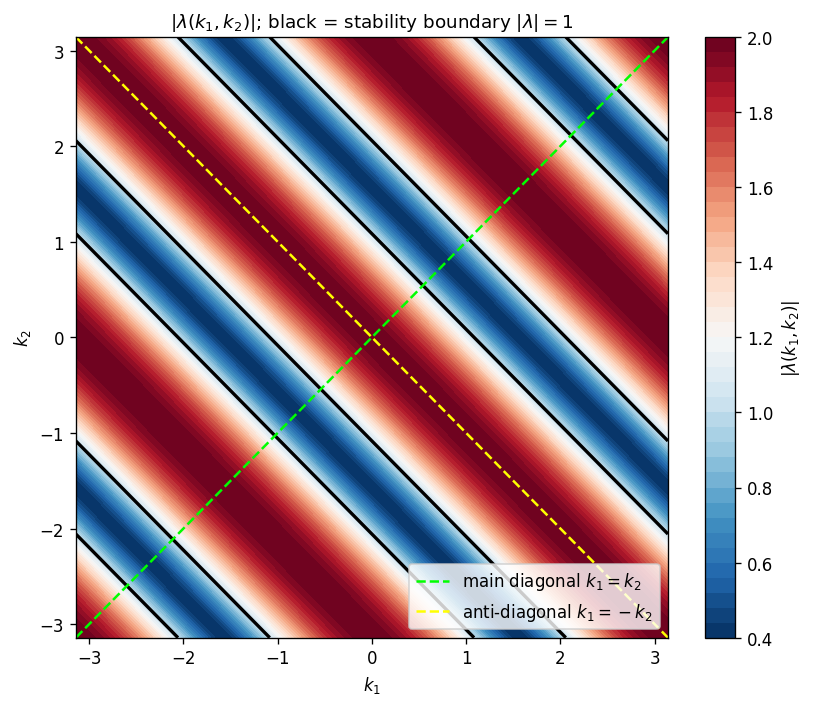
\includegraphics[width=0.74\textwidth]{book/assets/figures/intro/fig_amplification_map.png}
  \caption{A frequency-domain amplification map from the introductory cellular
  automaton example. Fourier thinking turns repeated translation-invariant
  updates into multiplication by frequency-dependent factors.}
\end{figure}

\section{Where This Fits}

The DFT is an explicit diagonalization. Convolution is a structured linear map.
The Fourier basis is the basis where that map becomes diagonal. This chapter is
therefore not a detour from the course; it is a concrete version of the main
story:
\[
  \text{choose a basis that reveals the map.}
\]

\begin{labbox}
Lab 11 explores image filters and edge detection. It can use larger image
libraries, but the book-level linear algebra is already visible in the small
NumPy examples here.
\end{labbox}

\section*{Chapter Summary}
\addcontentsline{toc}{section}{Chapter Summary}

\begin{itemize}
  \item Signals and images can be represented as vectors or matrices.
  \item Convolution with a fixed kernel is linear.
  \item Circular convolution is multiplication by a circulant matrix.
  \item Circulant matrices are diagonalized by the Fourier basis.
  \item The DFT turns convolution into pointwise multiplication.
\end{itemize}

\section*{Exercises}
\addcontentsline{toc}{section}{Exercises}
\subsection*{A. Theory}
\begin{exercise}\exerciseid{15.A1} State the spectral theorem for real symmetric matrices and explain why orthogonality is part of the conclusion. \end{exercise}
\subsection*{B. By Hand}
\begin{exercise}\exerciseid{15.B1} Compute the Rayleigh quotient of $\mat{2&0\\0&5}$ at $(1,1)$ and at $(0,1)$. \end{exercise}
\subsection*{C. Python / NumPy}
\begin{exercise}\exerciseid{15.C1} Sample random unit vectors and evaluate the Rayleigh quotient for a symmetric $2\times 2$ matrix. \end{exercise}
\subsection*{D. Challenge}
\begin{exercise}\exerciseid{15.D1} Explain why the maximum Rayleigh quotient of a symmetric matrix should be an eigenvalue. \end{exercise}

